\documentclass[10pt,a4paper]{article}
\usepackage[utf8]{inputenc}
\usepackage{amsmath}
\usepackage{amsfonts}
\usepackage{amssymb}
\usepackage{graphicx}
\usepackage{wrapfig}
\author{Flip van Spaendonck \& Lars Kuijpers \\ s4343123 \& s4356314}
\title{Compiler Construction Final Report}

\begin{document}
\maketitle
\tableofcontents

\section{Introduction}
For this course we've constructed a compiler from SPL to SSM language. We've chosen to program our compiler in Java, because we both have the most experience with it, and believe that its object structure might allow us to do certain things more intuitively than other programming languages. We've extended SPL with the ability to construct Muples and structs to it, which we will explain later on in the paper.

\subsection{The introduction of EXP}
For efficiency purposes we've decide to split the SPL grammar into two parts: EXP and SPL. EXP is the grammar we use to describe expressions and SPL is the rest. \\
\\
To prevent left recursion and make sure that every expression has the correct association, we've split the way expressions are represented in our syntax into different layers. This means that we don't have to worry afterwards about what operator binds more strongly than others, but it is included immediately in our grammar.\\
\\
There are a couple of other changes we made to the grammar. The first is how concatenation is notated in our language. Because concatenation is right-associative instead of left, it was impossible to prevent left-recursion, thus concatenation is always prefixed with an "\& " e.g.: We write \textbf{\& 1 : 3 : 4 : []} instead of \textbf{1 : 3 : 4 : []}.\\
\\
Another change is that we allow variable declarations to be written without an initial assignment. These kinds of declaration cause the variables to be assigned their type's corresponding "null-value" (int=0, char=the null character, bool=false and struct=null).\\
\\
Our final grammar for both EXP and SPL can be found in the appendix.

\section{Lexer}
The first part of our compiler is the lexer. The lexer takes the raw text input the user made in programming their SPL program and turns it into tokens, which will be used by later steps of the compiler.
\subsection{Basic structure}
Our lexer is based on the work shown in one of the practical sessions and made available on Blackboard. We've continued the work done there to include all inputs necessary to tokenize the SPL language (and our extensions). \\
\\
Our lexer accepts a string as an input, which will be saved locally. The lexer can then be asked for either the next token, or all next tokens with two seperate functions. With the nextToken() function, the lexer will skip any whitespace that is on its current position, until it finds another character. Depending on which character it finds, the function will return a specific token corresponding with that character. Sometimes determining which token to return requires looking at more than a single character, in which case the function will look at the next character in the input as well. If the next character is one of the expected ones, the function will return the corresponding token. If the character doesn't result in an expected combination with the one found previously, the lexer will halt and throw an error.\\
\\
The allNextTokens() function is an easy shorthand to loop through an entire input. This function will keep calling the nextToken() function, saving every returned token into a list. This loop will stop when nextToken() returns an End-of-file token. this token will be added to the list, and the result will be the return value of the allNextTokens() function.

\subsection{Special Tokens}
There are three cases where the lexer will (possibly) go further than one or two characters. These are numbers, words and comments.

\subsubsection{Numbers}
There are two cases in which the lexer will know it's looking at a number. The first one is when it simply finds a digit on the current position. It will then know it's a positive number, and keeps looking at the next character until it's not a digit anymore. If it finds a non-digit (or the current position is outside of the input), it will return a token with the value of the number, calculated with its digits and its sign (in this case positive).\\
\\
The other case where the lexer could be looking at a number is when the current character is a '-'. When this occurs, it will look at the immediate next character. If that next character is a digit, it will continue similarly as with positive numbers until it finds a non-digit or is out of bounds. It will then return a token with the value of the number, calculated similarly, but this time with a negative sign.

\subsubsection{Words}
If the lexer finds a alphabetical character, it knows it's looking at a word. Similarly to numbers, the lexer will continue looking at the next character as long as it's an alphabetical character or a digit. when it finds a character that is neither, it will stop and have an entire word. It then checks if the word is one of the designated keywords for SPL. If it is, it will return the correct token, depending on which keyword it is. If the word is not one of the designated keywords, the lexer will instead return a TokenIdentifier, which has the word as its value.

\subsubsection{Comments}
Comments are filtered out by the lexer. Whenever the nextToken function of the lexer finds the beginning of a comment (either '//' or '/*'), it will skip the contents of the comment and not tokenize anything that was in it. This is done similarly to how it skips whitespace. \\
\\
In the case of '//', the lexer will keep looking to the next character in the input, until it finds a newline character ('\textbackslash n'). After that, it calls nextToken() again, and will return the token that function call returns. This means it's able to handle multiple consecutive comments and will still always return a token (given there are no errors).\\
\\
In the case of '/*', the lexer will koop looking to the next character until it finds the characters '*/' consecutively. Similarly to with '//', after finding the '*/', the function will call nextToken() and return that function's return value. Since this happens on the lexer-level, there is nothing that checks if there is indeed a '*/' somewhere in the file. If there isn't any, the lexer will halt and throw an error.

%yada yada leest character voor character
%print en isempty zijn keywords
%comments worden niet doorgegeven


\section{Parser}
\subsection{Structure}
Now that we have the list of tokens corresponding to the program from the lexer, we can start running our parser on it. Our parser runs on a bottom-up architecture. To do this we first give the grammar/syntax of our (extended) SPL language to our compiler, which turns the syntax into a graph. This graph is used by the compiler to check which tokens are allowed at what point in the code.
\begin{figure}[h]
\centering
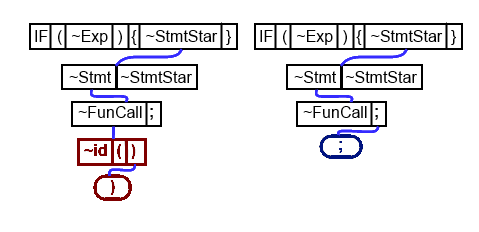
\includegraphics[width=280px]{TokenTraces.png}
\caption{Example of two tokentraces}
\label{fig:traces}
\end{figure}\\
If at some point during parsing there are no possibilities left, but there are still tokens left to be parsed, the compiler will give an error to the user, telling them that their code couldn't be compiled.\\
\\
When a token is allowed, it is mapped to a token-trace. \textit{(See figure \ref{fig:traces})} A token trace consists of a list of nested expressions, the token that was just parsed and a list of token-traces that cover the tokens left of this token in the code. So in the right trace in figure \ref{fig:traces} we have: a funcall (function call) inside a statement composition inside an if statement as the nexted expressions, the ";" as the current token and the token-traces that came before this one (including the token-trace on the left of the figure). \\
\\
Through this we can get a time-complexity of $\mathcal{O}(n \cdot k) $ with $n$ being the number of tokens in the code, and $k$ being the maximum amount of possible tokens that could follow a certain token. While n can of course vary per piece of code, $k$ is heavily influenced by how the syntax is written down.\\
\\
Once all tokens of the code have been parsed correctly and the last token-trace itself doesn't expect another token, we will have found a correct way of parsing the code. If multiple ways have been found of parsing the same code (this could happen for example when parsing an expression containing only a variable) the first possibility is taken. It is up to the structuring of the grammar itself to make sure that this can't lead to two possible parses with differing semantics.
\begin{wrapfigure}{r}{0.35\textwidth}
\centering
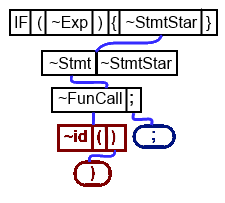
\includegraphics[width=120px]{TokenTree.png}
\caption{Part of a syntax tree consisting of the two token-traces described in \ref{fig:traces}}
\label{fig:tracetree}
\end{wrapfigure}\\
Now that we have a list of token-traces, the next step is putting them together into a single syntax tree \textit{(See figure \ref{fig:tracetree})}. No errors should be able to occur while the syntax tree is being constructed. Once we have constructed the syntax tree, we will convert it into a partially abstract syntax tree (pAST). This is done by creating a new AST whilst moving through the tree and checking for each node/expression whether it has an AST equivalent. If the node does have an equivalent AST node, this one is constructed and added to the new tree. If it does not have an equivalent, a copy of the original node is added to the new tree instead.

\subsection{Expression Optimization}
To reduce time-complexity we parse expressions separately. Before the above described parsing occurs, the code is first processed, detecting the locations of where an expression should be. E.g. when parsing "print 4+5*3;" the parser will detect the print keyword, which should have an expression after according to our grammar. The parser then takes all tokens between the print keyword and the next ";", in this case "4+5*3". The extracted tokens are then turned into custom expression tokens, which will be parses immediately using the EXP grammar/syntax. The parsed expressions will be checked for any redundant steps, i.e. "4+5*3" will always return 19, thus it is reduced to a simple constant, instead of the entire expression. This can only be done with certain expressions. In particular, an expression containing a variable can't be optimized fully. When the code is then parsed as described above, the syntax expects an expression token instead of an actual expression.
%expression optimization


\section{Semantic Analysis}
The next step in compiling our code will be semantic analysis. As previously described we've transformed our syntax tree into one with some AST nodes. The semantic analysis that will check if everything is well-defined and well-typed, and checks whether every non-void function will eventually hit a return statement.
\subsection{Type-checking and checking for well-definedness}
Checking if everything is well-typed and well-defined is done in the same step. We do this by traversing the tree and checking the following for each node:
\begin{itemize}
\item Whether the nodes declares anything new e.g., a Variable declaration.
\item Whether the node is well-typed.
\item Whether any undefined ID is used.
\end{itemize}
Each node has its own function to check whether it checks all of these marks, which will be called by the compiler during this tree traversal. E.g., for a variable declaration its own name is not allowed to be used in the declaration itself, while in the body of a function declaration it is allowed to use the function itself, such that recursive functions can be defined.\\
The IDs that are defined and their types are stored inside of an IDDeclarationBlock, this block is then passed through to the next node. If an ID is used but not declared a declaration exception is thrown. If something is incorrectly typed (for example an integer is assigned to a variable of type boolean, or an expression of type tuple is used in an if-statement) a type exception is thrown. If an exception is thrown the compiler stops compiling and gives the error to the user.
\subsection{Allocation of memory for code generation}
During the code generation step, when generating code for variables or function calls, it is necessary to know at what domain-level they are defined. When an ID (for a function call, variable or struct initialization) is encountered during Type-checking we check whether it's defined at the following levels of priority:
\begin{enumerate}
\item Local scope: These concern variables that are declared within a function's or constructor's body, and does not concern functions and constructors themselves.
\item Struct scope: This scope only exist when looking at code within a struct declaration (which we will explain in more detail when we talk about our extension). As you can not declare a new kind of struct inside of another struct declaration body, these are not found at this level.
\item Global scope: This concerns everything defined in the SPL code body (struct, variable and function declarations).
\end{enumerate}
To check at what level something is defined, we start at the local scope and end with the global scope. This means that if an ID is defined at both the global level and at the local level, the higher level \textit{(=local)} will take priority. It is not allowed to use the same id twice at the same level.\\
\\
The location where variables are stored depends on at what level the ID is declared. Variable addresses at local scope are temporary and are thus stored in the local memory. Variable addresses at struct and global scope are stored in the heap. Any variable addresses in the global environment or a specific struct are stored next to each other in memory (the same way a Muple would be stored; more on Muples in our extension). The address of this memory block is then stored in the local memory, see \ref{fig:linkmemory}.
\begin{figure}[h]
\centering
\begin{tabular}{c|c}
MP offset & what? \\\hline
0 & previous local memory address\\
1 & Heap address of global variable addresses\\
2 & Heap address of current struct variable addresses\\
3  & Temp variables\\
4 & Temp variables\\
\vdots & \vdots\\
n & Temp variables
\end{tabular}
\caption{local memory usage}
\label{fig:linkmemory}
\end{figure}
\subsection{Checking for termination}
Checking whether a non-void function will eventually hit a return statement is done at the moment its AST node is generated. During this generation, the function's body is traversed to check, given that it terminates, if it will eventually hit a return statement. Checking whether the return statement is of the correct type is done later, as described above.

%AST construction
%Monomorphic Type Checking


\section{Code Generation}
\subsection{Basic Structure} 
After the program has been checked for correctness, we can actually start generating the code. First, we'll talk about a couple of semantic choices we've made at this stage of our compiler. We decided that we wanted to approach variables on a by-reference basis. This is because we found it more intuitive to handle all kinds of variables in the same way, rather than (as would be the case with by-value lists and tuples) some are different and others aren't. We also chose to make the print function only print the value of basic types. For more complex data structures, such as lists, tuples and those from our extension, it will simply print the value of the memory address, rather than the value at that address itself.\\
\\
The way we do code generation is tied into the AST we made in our parser. Every node in the AST has a function called addCodeToStack(). This function has two arguments: the codestack and an incrementary counter. The codestack starts empty, and will eventually contain the entire SSM code for the program being compiled and put as return value for the function. The counter is used for the uniqueness of some labels, which we will talk about later. The idea of addCodeToStack() is that the node for which the function is called will add code that does something according to the type of node it is (for example, an addition node will generate code that adds something) and will also call the addCodeToStack() function for any of its children. The idea is to first evaluate the children, if need be, and then continue with their results on the memory stack. \\
\\
In the example used before, an Addition node would call addCodeToStack() its two children containing the arguments, and would itself add an 'add' to the codestack. When the SSM code will be runned, the two arguments will be evaluated first, and will end up on top of the memory stack, after which 'add' will be called, and the result on the memory stack will be the result of the addition.
%call-by-reference
%print only for basic types (otherwise as pointer)
%codestack (every node is verantwoordelijk voor zn eigen code)

\subsection{Data structures}
In the standard SPL we had two types of data structures: tuples and lists. These were both saved to memory in different ways. Tuples were saved as arrays are in many languages. Both items in the tuple are saved right next to each other in the memory. A difference from most languages is that, due to the way the SSM command we use to save tuples is implemented, making a tuple will return the address of the second item, not the first. This only really changes the code generated for the tuple accessors, .fst and .snd, as .fst now gets the value (and as we work by-reference, this value will be a reference address) of the tuple address minus 1.\\
\\
The way we use lists is similar to linked lists in Java. Every item in the list consists of what is essentially a tuple. The first item in a tuple is the value (once again, this will be a reference address) of the place in the list corresponding to the number of the tuple. So for the first tuple, the value here will be the first value in the list, the second tuple will contain the second value, etc. The second item in the tuple will be a reference address to the next tuple in the list. If this tuple is the last, it will point to 0. As there can never be a tuple entry at memory address 0 (because that's where the code is saved), we know for certain that this is the last tuple in the list.
%tuples/lists

\subsection{Variables}
When looking at how variables are used in SPL, we can differentiate between two types of usage: allocation and variable calls.
\subsubsection{Allocation}
This is when a value needs to allocated to a variable. This occurs either through an assignment or a variable declaration and only occurs at the level of the SPL grammar, not at the EXP level.\\
\\
For these two cases the expression on the right is evaluated using the addCodeToStack() function, and will then stored on the heap. In the case of a variable declaration, the value is added to the heap and the heap address will be saved in the location allocated to that variable during type-checking. In the case of an assignment, the allocated location's address is first loaded in, and then stored using the corresponding instruction. As the location (heap or local) is known at compile time, no decision making will have to happen during run-time.
\subsubsection{Variable calls}
This is when a variable is called upon to get the value that it represents (e.g. "print dog" in which the value of dog is requested so that it can be used in print). These can be found under the EXP grammar.\\
\\
When a variable is called upon during an expression, the address of the value is put on the stack using the code generated with addCodeToStack(). When we check whether the ID is well-defined, we will also know where it should be stored (either on the heap or locally) and thus we will know whether to use \textit{"ldh"} or \textit{"ldl"} respectively.
%variables

\subsection{Functions}
Functions only have to be executed whenever they are called, so their SSM code is generated separately. Whenever the compiler finds a function in the SPL program, it will add any variable declarations at the start of the function body to the current domain. Any global variables with the same name as local variables will be overwritten by the local variables, and put back once the compiler finds a return statement. The code for the rest of the function body is generated by calling addCodeToStack() on the node of the body itself. This block of code is then given a label corresponding to the function name, and this entire thing is added to the SSM codestack.\\
\\
Whenever a function is called, it will jump to the label corresponding to the name, save the PC where it left from and the function code will be executed. This will work as any other function code, until it reaches a Return. When the return is reached, two things can happen. If the function has a return-type of null, it will simply remove any local variables from the memory and jump back to the saved PC+1, continuing the code where it left off. If the function has any other return-type, it will do the same, but instead of removing all local variables, it will leave the return value on top of the stack after its return, so this value can be used in the rest of the program.
%function calls


\section{Extension}
\subsection{Idea}
The idea behind our extension to SPL is to allow for more complex data structures to be determined than only tuples and lists. We thought that the ability to define more complex data would help users to make more intuitive programs for problems were this might be relevant. We've decided to add two things: n-ary tuples, which we call Muples and structs. 
\subsection{Muples}
Muples are quite simply tuples that can have any number of items, not just two. The size of a Muple is still known and set at compile time, so they can't be changed at runtime. The implementation of Muples is also very similar to our implementation of tuples; all items in a Muple are right next to each other in the memory. A Muple is created in the same way a tuple is, but the declaration can be arbitrarily large. To access Muple fields, we've added a new field-accessor: .[n]. By using Muple.[n], the nth value of the Muple will be returned. Since Muples only add functionality, they have fully replace tuples in our implementation of SPL, and the accessor functions .fst and .snd are not used anymore.
\subsection{Structs}
%extension idea + motivation
The second aspect we added to SPL with our extension is the idea of structs. Structs are similar to classes in Java or object in other OO programming languages. Structs are user-defined blocks of variable and function definitions. Every struct has to have a single constructor, which is a function that returns the struct type itself. By calling this constructor, the user can create an instance of a struct.\\
\\
A struct has to be initialized before it can be used, and can have multiple instances at a time. From these instances of a struct, the user can call the variables or functions that struct type has. With structs we have introduced a new scope between local and global, namely the struct level. Whenever a variable or function is called for a struct, it will be called in the domain of that struct. As mentioned in the section about type-checking, the type checker actually checks to which scope any function or variable call belongs and makes sure this goes right.\\
\\
The way structs are implemented is mostly based on the way we implement similar things. The functions of a struct are added to the code in much the same way that 'normal' or global functions are added. The compiler knows which one to call at which point because of the type-checker, as mentioned before. The variables of a struct are stored similarly to the global variables: in a single Muple that is stored in the heap. Whenever a variable is called from the struct, the correct one will be extracted from this Muple.\\
\\
It's also possible to include the new 'this' keyword in any expression that is within a struct. If the this keyword is outside of a struct, the parser will throw an error (much like when return is found outside of a function). 'This' will give the struct instance that is the current domain back as a variable, so the instance can be used in its own body.

\appendix
\section{SPL Grammar}
\begin{math}
\centering
\begin{aligned}
SPL =& \text{ Decl+}\\
Decl  =& \text{ VarDecl}
 \\&| \text{ FunDecl }
 \\&| \text{ StructDecl}\\
VarDecl =& \text{ Type id [ '=' EXP ] ';'}\\
FunDecl =& \text{ id '(' [ FArgs ] ')' '::' FunType '\{' VarDecl* Stmt+ '\}' }\\
FArgs =& \text{ id }
 \\&| \text{ id ',' FArgs}\\
FunType =& \text{ Type* '-$>$' RetType}\\
RetType =& \text{ Type}
 \\ &| \text{ 'void'} \\
StructDecl =& \text{ id '\{' VarDecl* Constructor FunDecl* '\}'}\\
Constructor =&\text{ id '(' [ CArgs ] ')' '\{' VarDecl* Stmt* '\}' }\\
CArgs =& \text{ Type id }
 \\&| \text{ Type id ',' CArgs}\\
Type =& \text{ 'Bool'}
 \\&| \text{ 'Int'}
 \\&| \text{ 'Char'}
 \\&| \text{ '(' Mype ')'} 
 \\&| \text{ '[' Type ']'} 
 \\&|\text{ id }\\
Mype =&\text{ Type}
 \\&|\text{ Type ',' Mype}\\
Stmt =&\text{ 'if' '(' EXP ')' '\{' Stmt* '\}' ['else' '\{' Stmt* '\}']}
 \\&|\text{ 'while' '(' EXP ')' '\{' Stmt* '\}'}
 \\&|\text{ id Field* '=' EXP ';'}
 \\&|\text{ FunCall ';'}
 \\&|\text{ 'print' EXP ';'}
 \\&|\text{ 'return' [ EXP ] ';' }\\
Field =&\text{ '.' ('hd' $|$ 'tl' $|$ id $|$ '[' int ']' ) }\\
FunCall =&\text{ id '(' [ ActArgs ] ')'} \\
ActArgs =&\text{ EXP }
 \\&|\text{ EXP ',' ActArgs }
\end{aligned}
\end{math}
\section{EXP Grammar}
\begin{math}
\begin{aligned}
EXP =& \text{ BoolExp2}
 \\&|\text{ NumRng} 
 \\&|\text{ SetExp }
 \\&|\text{ '(' Mexp ')'}
 \\&|\text{ 'null'}\\
Mexp =& \text{ EXP [ ',' Mexp ]}\\
BoolExp2 =& \text{ BoolExp1 ('\&\&' $|$ '$||$') BoolExp2}
 \\&|\text{ NumRng ('==' $|$ '!=' $|$ '$<$' $|$ '$>$' $|$ '$<$=' $|$ '$>$=') NumRng}
 \\&|\text{ BoolExp1}\\
BoolExp1 =& \text{ [ '!' ] BoolExp0}\\
BoolExp0 =& \text{ 'True'}
 \\&|\text{ 'False'}
 \\&|\text{ CallUp Field }
 \\&|\text{ '(' BoolExp2 ')'}\\
NumRng =& \text{ NumFld ('+' $|$ '-') NumRng}
 \\&|\text{ NumFld}\\
NumFld =& \text{ Neg ('\%' $|$ '/' $|$ '*') NumFld}
 \\&|\text{ Neg}\\
Neg =& \text{ [ '-' ] NumSng}\\
NumSng =& \text{ int}
 \\&|\text{ char }
 \\&|\text{ CallUp Field}
 \\&|\text{ '(' NumRng ')' }\\
CallUp =& \text{ id}
 \\&|\text{ 'this' }
 \\&|\text{ FunCall }
 \\&|\text{ 'new' id '(' [ ActArgs ] ')' } \\
Field =&\text{ '.' ('hd' $|$ 'tl' $|$ id $|$ '[' int ']' $|$ FunCall) }\\
FunCall =&\text{ id '(' [ ActArgs ] ')'} \\
ActArgs =&\text{ EXP }
 \\&|\text{ EXP ',' ActArgs }
\end{aligned}
\end{math}
\end{document}